\chapter{Атомная отрасль}

\begin{figure}[h]
	\begin{center}
		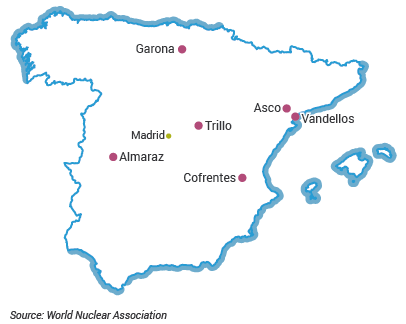
\includegraphics[width=.5\columnwidth]{./img/world_n_a.png}
	\end{center}
	\caption{АЭС Испании}
	\label{pic:mapOfNPP}
\end{figure}

Как видно из рис \ref{pic:mapOfNPP} атомные электростанции страны расположены в основном в центральной и восточной части государства. Это связано с развитием промышленности страны, которая нуждается в дополнительном объеме электроэнергии.

\section{Предыстория развития атомной энергетики}

Реализация ядерной программы началась в середине 1960-х годов с почти синхронного внедрения сразу трех типов реакторных технологий: с водой под давлением, кипящей и газографитовой. В 1964–1968 годах началось строительство трех атомных станций, использующих эти технологии, в разных частях страны:
\begin{enumerate}
	\item АЭС «Хосе-Кабрера» (она же «Сорита») с реактором PWR — недалеко от столицы страны, в регионе (так называемом автономном сообществе) Кастилия —Ла-Манча
	\item  АЭС «Санта-Мария де Гаронья» с реактором BWR — в Кастилии и Леоне, около границы со Страной Басков
	\item АЭС «Бандельос» с газоохлаждаемым реактором — в Каталонии.
\end{enumerate}  

По одному блоку на каждой из этих площадок вошли в строй в 1969–1972 годах. В то время уровень развития науки и промышленности в Испании был недостаточен для создания собственных реакторных технологий, которое могли себе позволить некоторые другие неядерные державы, такие как Канада, Япония, Швеция, Германия, Италия. Атомная энергетика Испании с самого начала опиралась исключительно на зарубежные, преимущественно американские технологии, что предопределило ее современный облик: все строившиеся в этой стране энергетические реакторы, кроме двух, поставлены компаниями США (а именно Westinghouse и General Electric).

Последовательность построения и эксплуатации АЭС на территории Испании:
\begin{enumerate}
	\item Хосе Кабрера - 1969 год, реактор типа PWR с мощностью 141 МВт.
	\item Санта-Мария де гаронья - 1971 год. Тип реактора BWR 446 МВт
	\item Бандельос  №1 - 1972 год. Тип реактора газографитовый  480 МВт
	\item Альмарас №1 - 1983 год. Тип реактора PWR 1011 МВт
	\item Альмарас №2 - 1984 год. Тип реактора PWR 1006 МВт
	\item Аско №1 - 1984 год. Тип реактора PWR 995 МВт
	\item Конфрентес - 1985 год. Тип реактора BWR 1064 МВт
	\item Аско №2 - 1986 год. Тип реактора PWR 997 МВт
	\item Бандельос №2 - 1988 год. Тип реактора PWR 1045 МВт
	\item Трильо - 1988 год. Тип реактора PWR 1003 МВт.   
\end{enumerate}

\begin{figure}[h]
	\begin{center}
		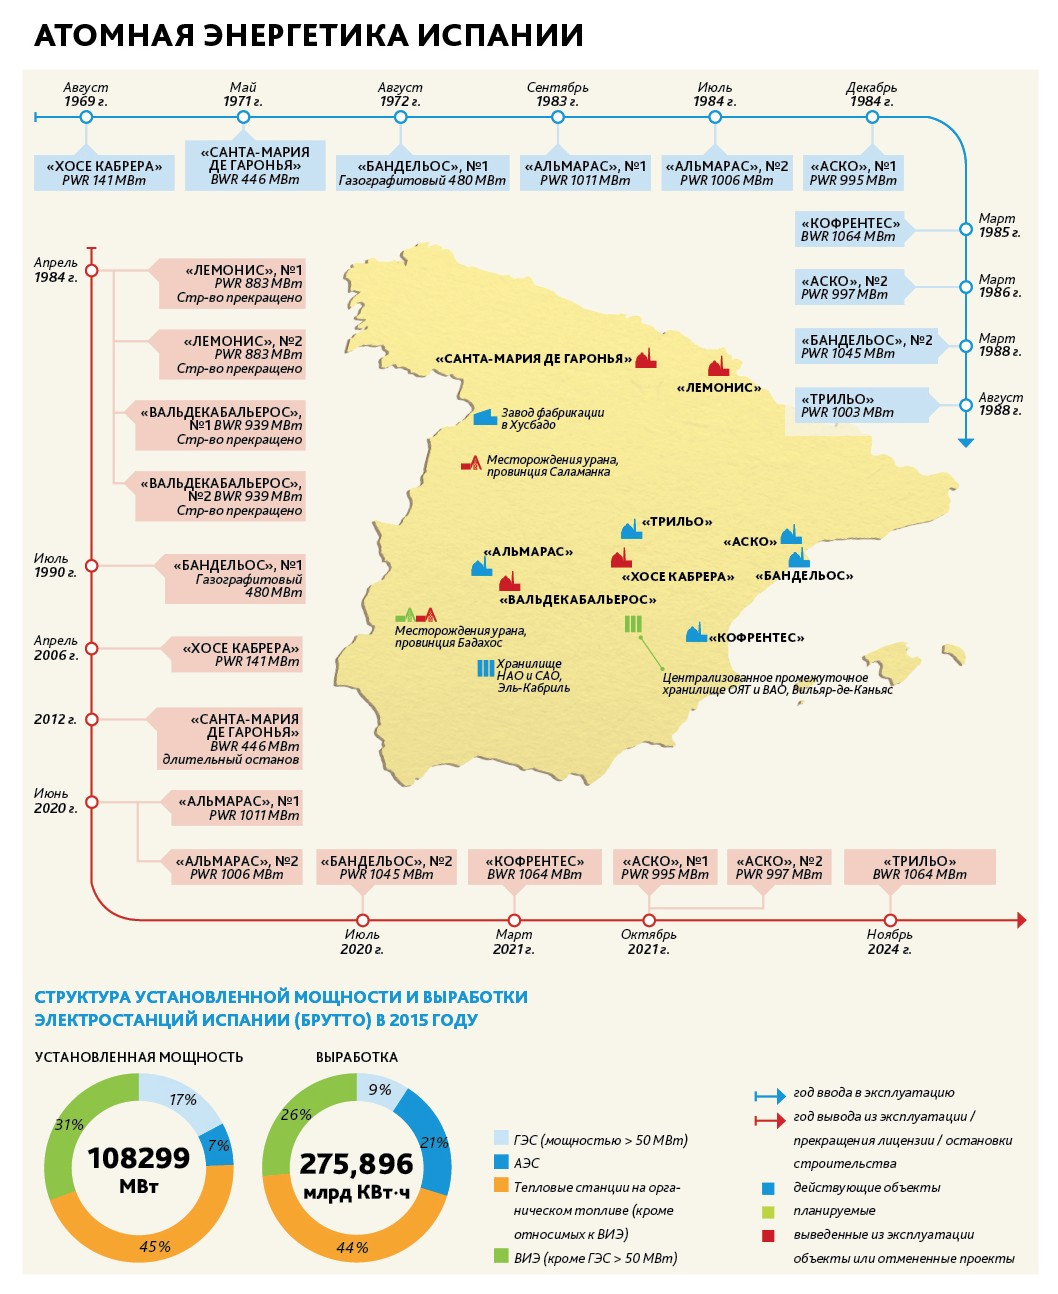
\includegraphics[width=.5\columnwidth]{./img/spain_en_history.jpg}
	\end{center}
	\caption{Хронологическая последовательность развития АЭС на территории Испании 2016}
	\label{pic:spain_en_history}
\end{figure}